\section{Entraînement avec les hyperparamètres optimaux}%
\label{sec.results.retrain}

Après le réglage des hyperparamètres, nous avons entraîné le modèle en spécifiant un nombre maximal d'époques de 20.
L'entraînement s'est arrêté après 9 époques à cause du rappel de fonction \verb|EarlyStopping|,
car le score \gls{bleu} sur le corpus de validation n'a pas augmenté pendant 3 époques consécutives.
L'exécution a duré 1~h~26~min~27~s.

\begin{figure}[!hbt]
    \begin{subfigure}{.5\textwidth}
        \caption{Exactitude}
        \begin{center}
            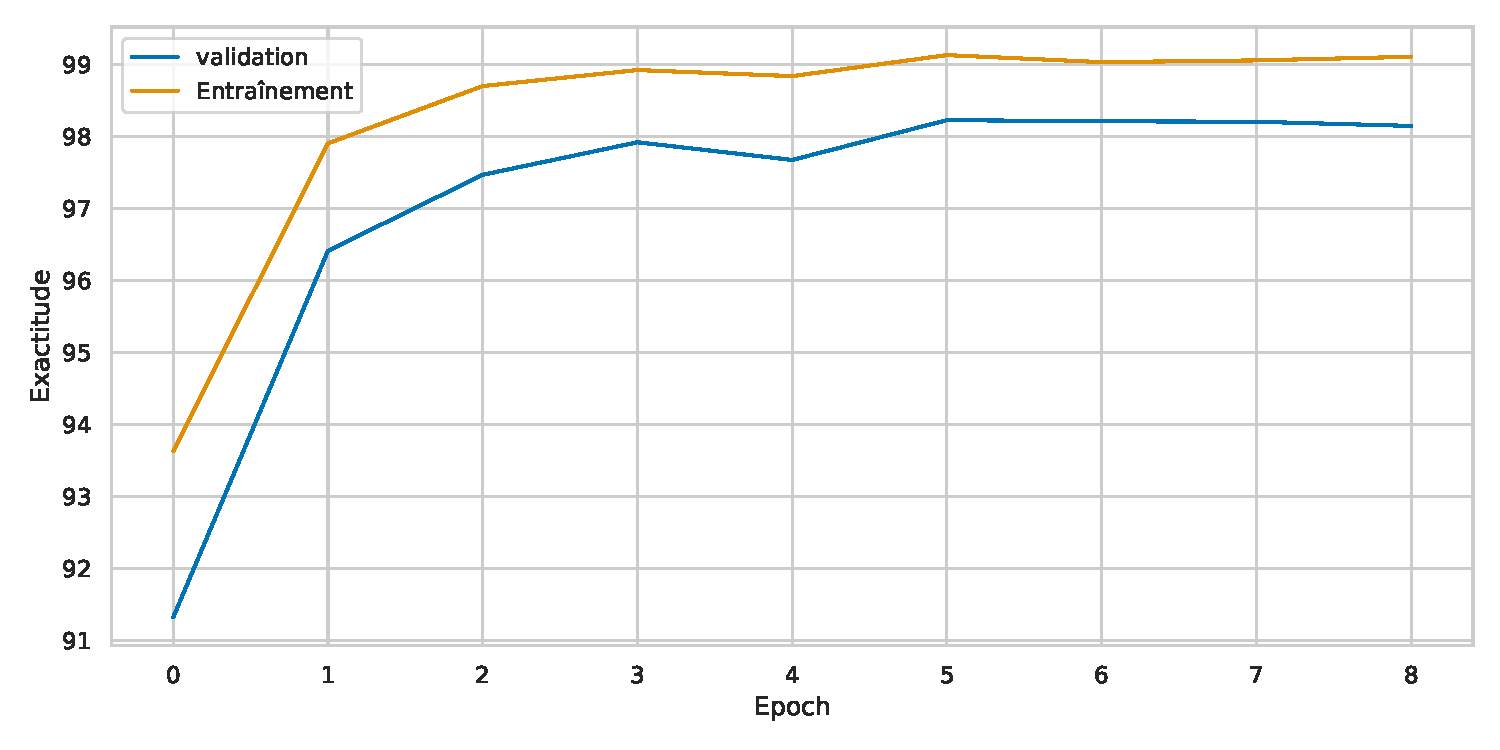
\includegraphics[width=\textwidth]{assets/python/tuned-accuracy.pdf}
        \end{center}
        \label{fig.results.tuned.training.accuracy}
    \end{subfigure}
    \begin{subfigure}{.5\textwidth}
        \caption{\glsfmtshort{bleu}}
        \begin{center}
            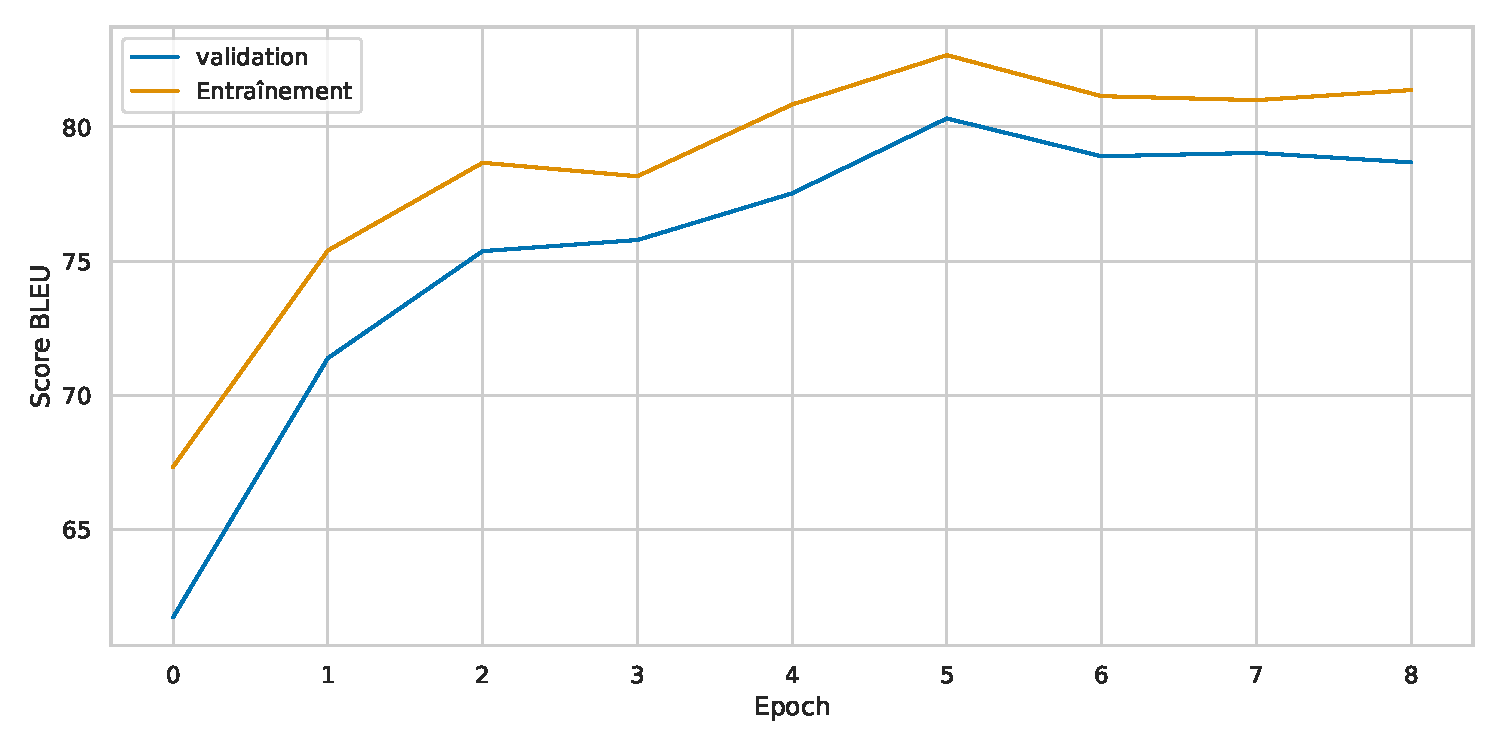
\includegraphics[width=\textwidth]{assets/python/tuned-bleu.pdf}
        \end{center}
        \label{fig.results.tuned.training.bleu}
    \end{subfigure}
    \begin{subfigure}{.5\textwidth}
        \begin{center}
            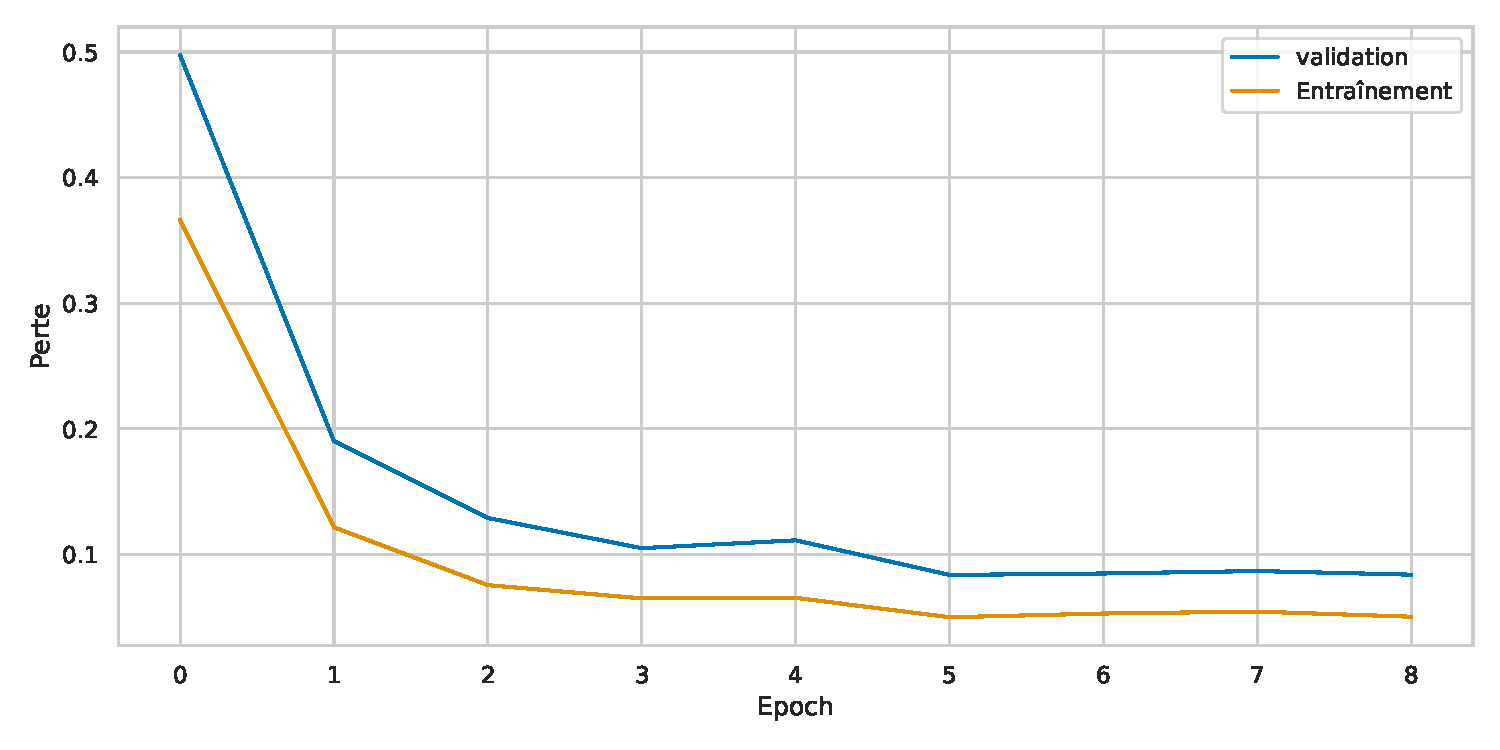
\includegraphics[width=\textwidth]{assets/python/tuned-loss.pdf}
        \end{center}
        \caption{Perte}
        \label{fig.results.tuned.training.loss}
    \end{subfigure}
    \caption{Évolution des métriques avec les hyperparamètres optimaux.}
    \label{fig.results.tuned.training}
\end{figure}

Les courbes d'apprentissage sont présentées sur la Figure~\ref{fig.results.tuned.training}.
On remarque que les métriques d'entraînement et de validation sont très fortement corrélées.
Il est donc improbable que le modèle sur-apprenne sur le corpus d'entraînement.
La meilleure valeur du score \gls{bleu} a été obtenue après 6 époques et elle vaut 80.32\%.

Sur le corpus de test, le score \gls{bleu} est de 79.61\%, 
l'exactitude est de 98.15\% et la perte de \(8.39\cdot 10^{-2}\).
Cela indique que le modèle généralise bien et qu'il n'a pas surappris sur les corpus d'entraînement et de validation.
Comparé à la valeur de base présentée dans la Section~\ref{sec.results.corpus},
le score \gls{bleu} a augmenté de 16.89\%.
Une amélioration de 2.22\% a été obtenue par rapport au modèle entraîné avec les hyperparamètres par défaut.

